% DRAFT (BD) for the BD regions of devopsSre.tex (rows 4, 6, 7, 8). Labels follow the skeleton (bd-drafts/devopsSre-skeleton.tex).
% Paths assume the manual repo layout: evidence/NNN-... (BD's evidence 140-167 must be copied there) and config/monitoring/grafana/...
% Before moving into the manual repo:
%   - copy evidence 140-167 (the files named below) into evidence/
%   - copy monitoring/grafana/group1-sre-dashboard.json and alert-rules.yaml to config/monitoring/grafana/ (and to infra/monitoring/grafana/ by PR)
%   - replace every \Todo / \StatusPending below once the item is done (normal-build comparison, issues, version 1.3, final build).
% Points per the course rubric (sec. 5.5): row 4 = 15, row 6 = 15, row 7 = 10, row 8 = 10.

% ===== BD region: row 4 =====
% Region: sreDashboard (single owner; edit only your own region)
\section{Dashboard (15 points)}\label{Section:sreDashboard}
\textbf{Owner:} BD. \textbf{Status:} dashboard built and checked November 11, 2026; normal-build comparison \StatusPending.

\paragraph{Dashboard and data source.} The dashboard \emph{Group 1 Startup Server (SRE)} was imported into Grafana from a
JSON file (\texttt{config/monitoring/grafana/group1-sre-dashboard.json}), after the Prometheus data source was added with the
private address \texttt{http://prometheus:9090} (inside the Grafana container, \texttt{localhost} is Grafana itself, not Prometheus).
The time zone is fixed to \texttt{America/New\_York} (shown as EST), the default range is the last 3 hours, and the page refreshes every 30~s
(the scrape interval). Thresholds are drawn as lines on the panels and legends are on. The dashboard definition is kept as JSON in Gitea
\Todo{link to the infra pull request that adds monitoring/grafana/}, because screenshots alone cannot restore a dashboard.
\FigRef{145} and \FigRef{146} show the result; the first copy was deleted and imported again after the scrape-health table was widened.

\begin{figure}[htbp]
\centering
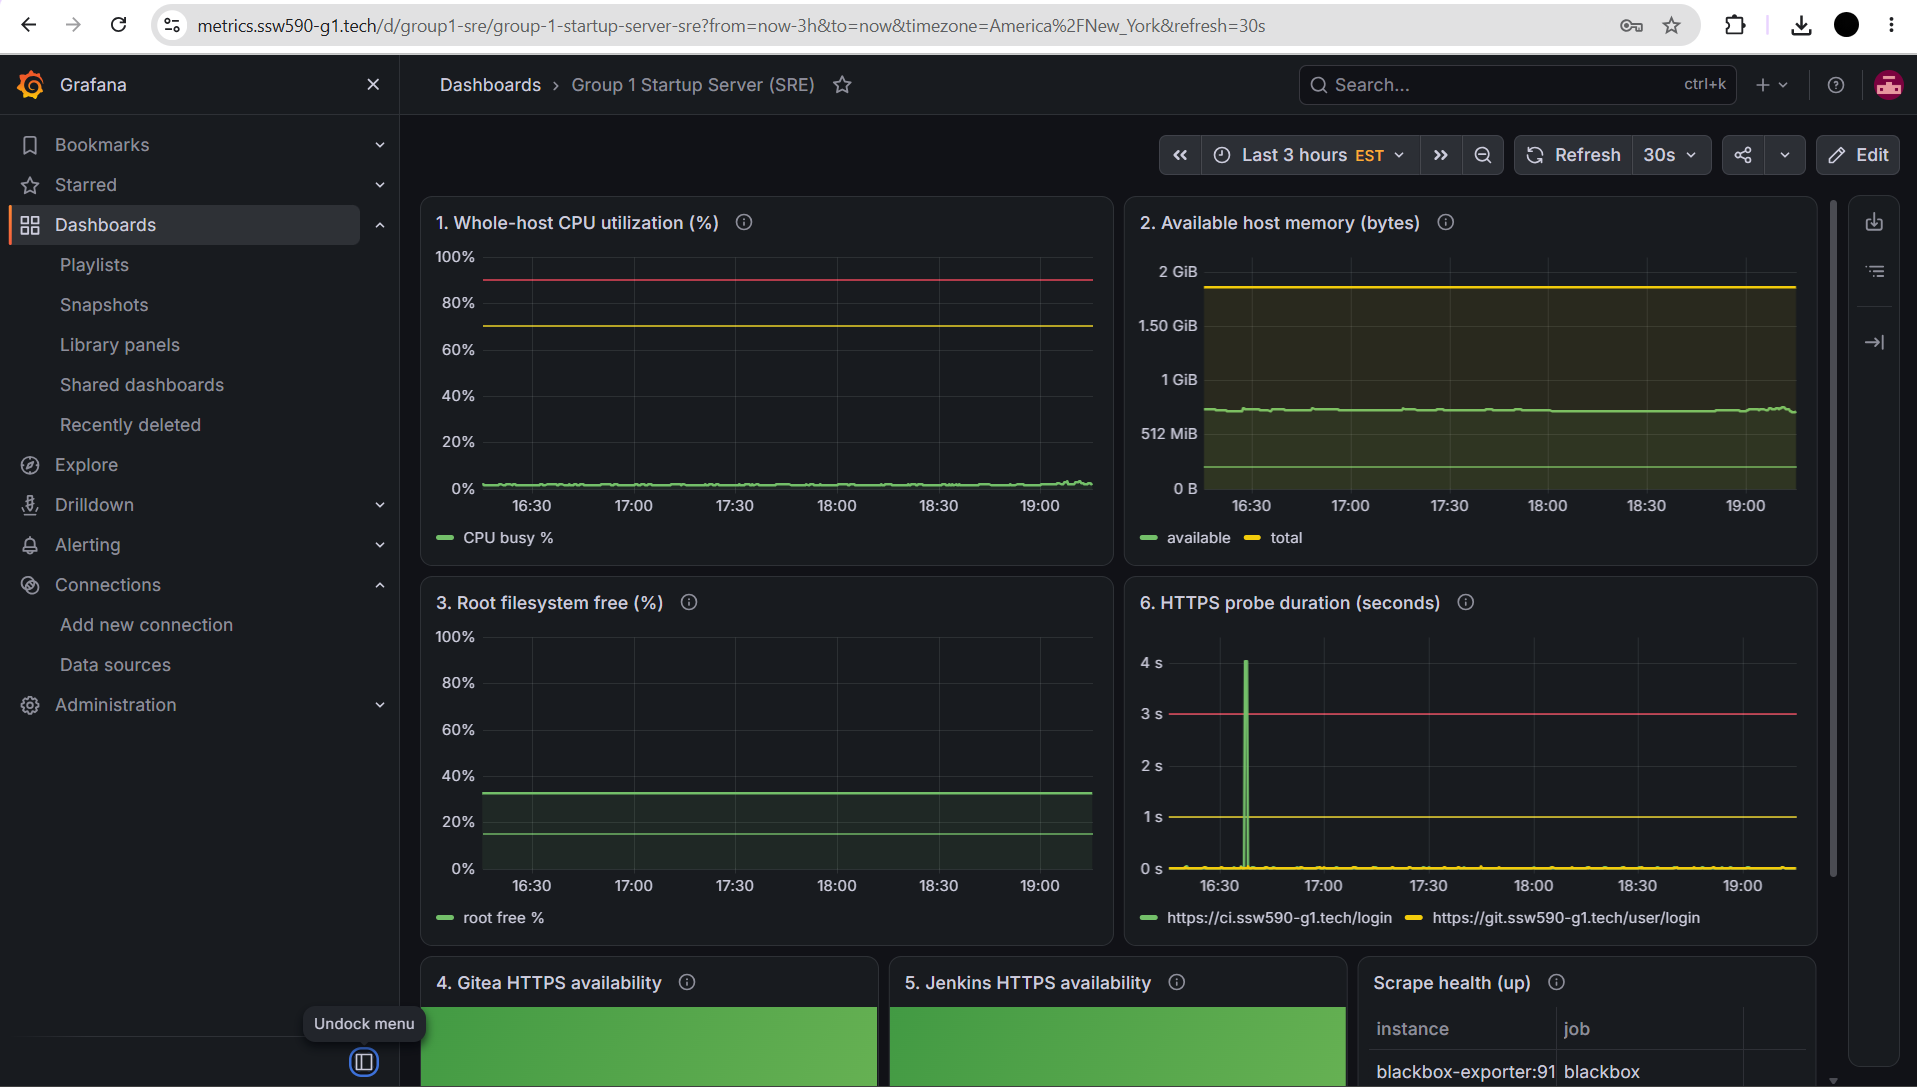
\includegraphics[width=\linewidth]{evidence/145-grafana-dashboard-group1-sre-panels-1-2-3-6-top-half-bd-2026-11-11.png}
\caption{Dashboard, top half, November 11, 2026, last 3 hours EST: CPU about 2\%, available memory about 750~MiB of 1.86~GiB, root filesystem free about 33\%, probe duration of both URLs (one 4~s sample on the Jenkins line).}
\label{Fig:E145}
\end{figure}

\begin{figure}[htbp]
\centering
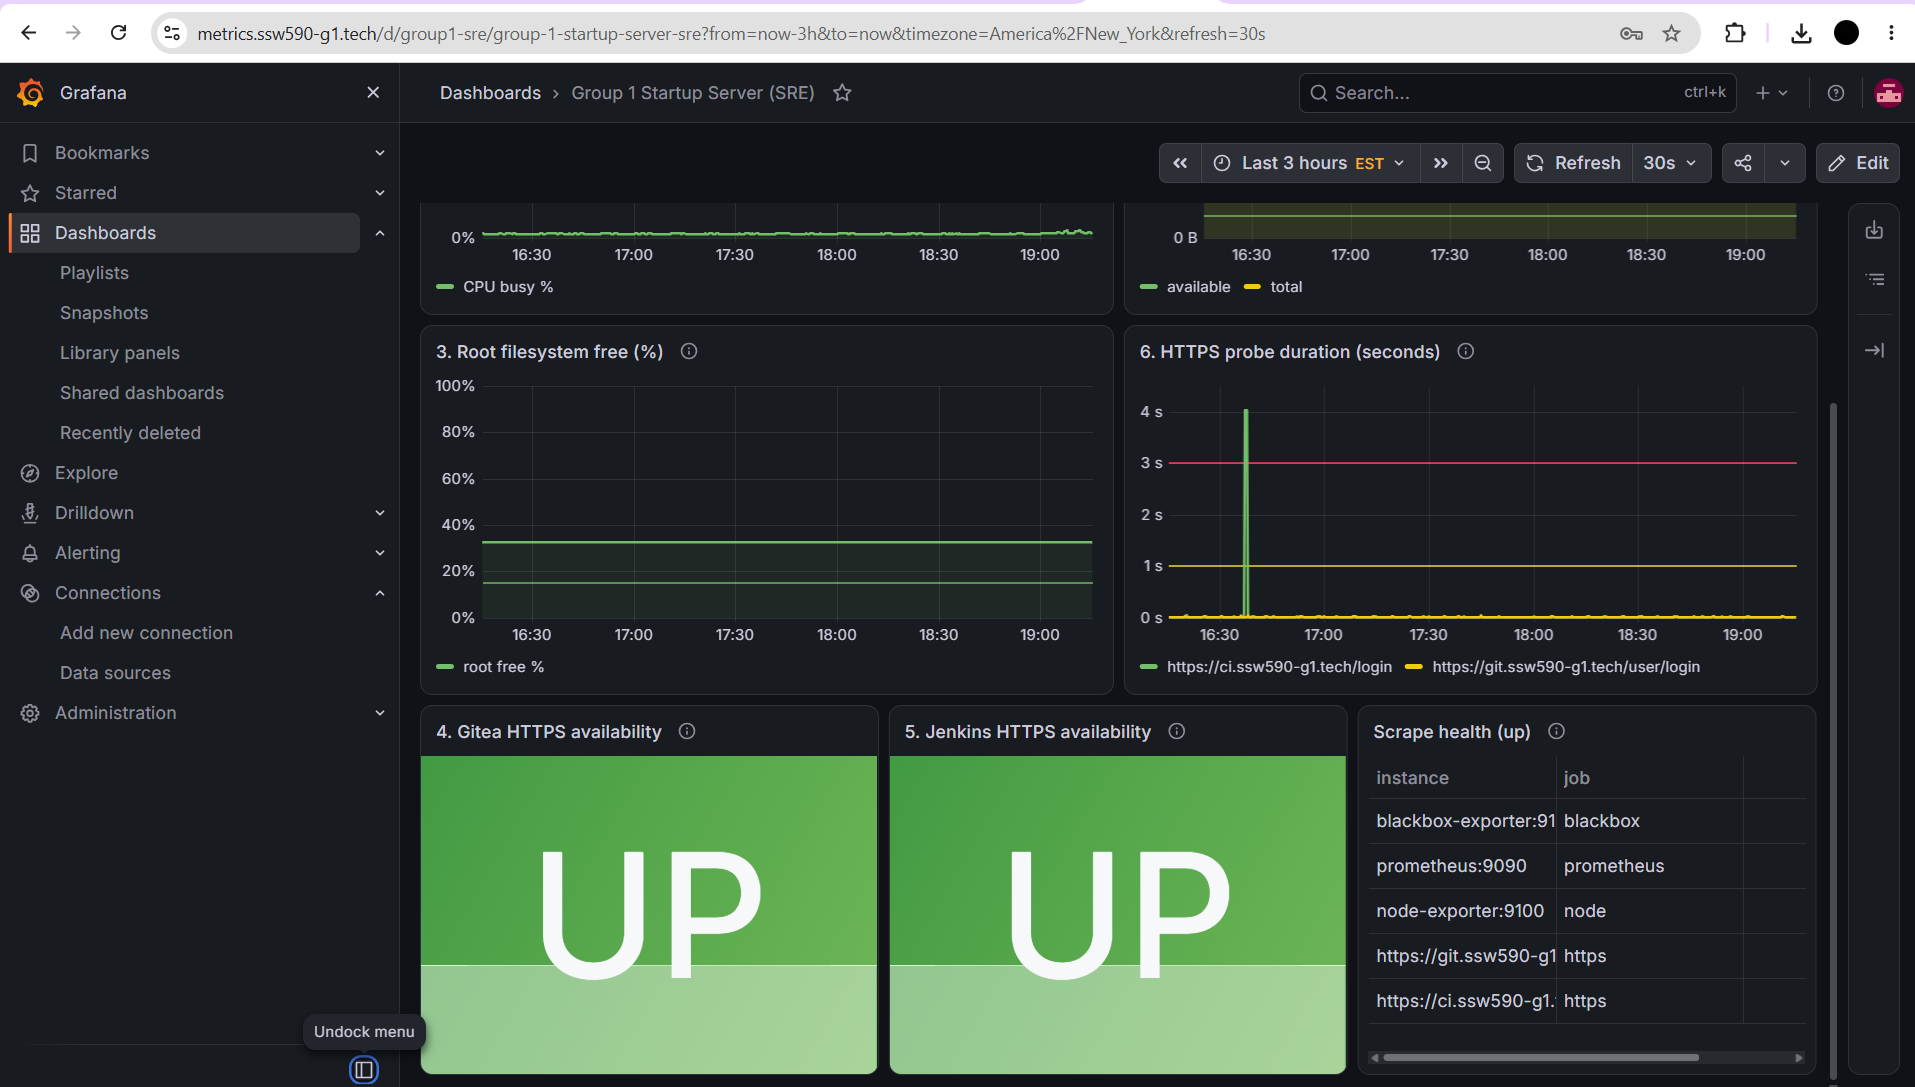
\includegraphics[width=\linewidth]{evidence/146-grafana-dashboard-group1-sre-panels-3-4-5-6-scrape-health-bd-2026-11-11.png}
\caption{Dashboard scrolled down: Gitea and Jenkins both UP, probe duration with two labeled lines, and the scrape-health table.}
\label{Fig:E146}
\end{figure}

\paragraph{The six required panels and their queries.} Each query was run against Prometheus' own API before it went into the
dashboard and compared with \texttt{free -b} and \texttt{df -B1 /} (\ListRef{142}).

\begin{tabularx}{\linewidth}{L{0.6cm}L{3.6cm}Y}
\caption{Dashboard panels and why their queries are written this way\label{Table:SrePanels}}\\
\toprule \textbf{\#} & \textbf{Panel (unit)} & \textbf{Explanation of the query (the queries are in \ListRef{SreQueries})}\\ \midrule
\endfirsthead
\toprule \textbf{\#} & \textbf{Panel (unit)} & \textbf{Explanation}\\ \midrule
\endhead \bottomrule \endlastfoot
1 & Whole-host CPU utilization (percent) & The CPU time counter grows forever, so its rate over 2 minutes is the idle share per second; the average over both CPUs is the host-wide idle share, and 100 times one minus it is the busy percentage. Whole host, not per container.\\
2 & Available host memory (bytes, IEC) & The kernel's estimate of memory applications can still get; it is not the \emph{free} figure. Same value as the \emph{available} column of \texttt{free -b}. Total memory is a second line.\\
3 & Root filesystem free (percent) & Available bytes divided by the size of the same series, the real root filesystem \texttt{/dev/nvme0n1p1} (xfs). The other filesystems (\texttt{/boot/efi}, \texttt{/run}, \texttt{/tmp}) are not mixed in.\\
4 & Gitea HTTPS availability (0 or 1) & 1 means DNS, TLS verification, allowed redirects and the final status all passed. A login-page probe does not prove a Git push.\\
5 & Jenkins HTTPS availability (0 or 1) & The same for the Jenkins login URL; \texttt{/login} is the page Jenkins shows to everyone.\\
6 & HTTPS probe duration (seconds) & One labeled line per URL; a slow response shows before a failure.\\
\end{tabularx}

\begin{longlisting}
\begin{minted}[fontsize=\scriptsize]{text}
1 CPU %      100 * (1 - avg(rate(node_cpu_seconds_total{mode="idle"}[2m])))
2 memory     node_memory_MemAvailable_bytes            (and node_memory_MemTotal_bytes)
3 root free  100 * node_filesystem_avail_bytes{mountpoint="/",fstype!~"tmpfs|overlay|squashfs"}
                 / node_filesystem_size_bytes{mountpoint="/",fstype!~"tmpfs|overlay|squashfs"}
4 Gitea      probe_success{job="https",instance="https://git.ssw590-g1.tech/user/login"}
5 Jenkins    probe_success{job="https",instance="https://ci.ssw590-g1.tech/login"}
6 duration   probe_duration_seconds{job="https"}        (legend: {{instance}})
table        up
\end{minted}
\caption{The dashboard queries (Prometheus query language), as saved in the dashboard JSON.}
\label{Listing:ESreQueries}
\end{longlisting}

The scrape-health table uses \texttt{up}: \texttt{up} is 1 when Prometheus could scrape the target, while \texttt{probe\_success} can be 0 although \texttt{up}
is 1 (the collection worked, the probed request failed). \ListRef{142} lists every filesystem Node Exporter reports and why only the xfs root is used.
Values at 03:29~UTC: CPU 1.69\%, available memory 805,617,664 bytes (\texttt{free}: 806,154,240), root free 32.94\% (7,047,094,272 of 21,395,124,224 bytes),
both probes 1 with 0.012~s and 0.040~s.

\begin{longlisting}
\inputminted[fontsize=\scriptsize]{text}{evidence/142-dashboard-queries-checked-against-prometheus-and-host-bd-2026-11-10.txt}
\caption{Each dashboard query run against Prometheus and compared with \texttt{free -b} and \texttt{df -B1 /}, November 10, 2026 (real output).}
\label{Listing:E142}
\end{longlisting}

\paragraph{Normal Jenkins build.} One normal run of the existing pipeline was captured on a calm server: build \#3 of
\texttt{twintrack/main}, started by BD with \emph{Build Now} on November 12, 2026 at 01:41:47~UTC (November 11, 20:41:47~EST), commit
\texttt{a0094a8} (the merged pull request \#10), result SUCCESS, duration 2.4~s, end about 01:41:49. The console says
\texttt{Running on Jenkins in /var/jenkins\_home/workspace/twintrack\_main}: the build ran on the \emph{controller}, so its resource
use is inside this host's measurements (\FigRef{169}). Jenkins had been up for 14 minutes since its restart in the outage test.
The host values come from Node Exporter's raw samples, one every 30~s (\ListRef{168}):

\begin{tabularx}{\linewidth}{L{3.2cm}L{3.4cm}L{2.6cm}Y}
\caption{Host CPU and available memory around build \#3 (UTC, 30~s samples)\label{Table:SreBuildSamples}}\\
\toprule \textbf{Sample} & \textbf{CPU busy, previous 30~s} & \textbf{Available} & \textbf{Position}\\ \midrule
\endfirsthead
\toprule \textbf{Sample} & \textbf{CPU busy, previous 30~s} & \textbf{Available} & \textbf{Position}\\ \midrule
\endhead \bottomrule \endlastfoot
01:40:46 & 5.7\% & 675~MiB & before\\
01:41:16 & 6.7\% & 671~MiB & before\\
01:41:46 & 5.4\% & 662~MiB & before (1~s before the start)\\
01:42:16 & 10.1\% & 654~MiB & during: the only sample containing the build\\
01:42:46 & 6.2\% & 662~MiB & after\\
01:43:16 & 4.5\% & 695~MiB & after\\
\end{tabularx}

\emph{What changed:} the one sample that contains the 2.4~s build reads 10.1\% CPU, against 4 to 7\% before and after. A one-core job of 2.4~s adds about
$2.4/(30\times 2)=4$ percentage points to a 30~s average over two CPUs, so the rise is of the size expected, but it is a single sample whose neighbours already
vary between 3 and 7\%, so it is consistent with the build and does not prove it. \emph{What did not change:} available memory moved by 10 to 40~MiB, within
the normal movement of the minutes before (632 to 678~MiB). \emph{Why so little is visible:} a build of 2.4~s falls inside one 30~s scrape and is averaged with
27 quiet seconds; the pipeline is two short Python commands. No extra load was created to force a spike. Whole-host figures do not say how much of the CPU belongs to
Jenkins rather than to another container. Other activity in the window (the manual build on the Gitea Actions runner at 01:35 to 01:36 with CPU above 50\%, and a missing
sample at 01:38:46) is listed in \ListRef{168}.
The earlier build \texttt{main} \#2 (01:29:12~UTC, 7.9~s, \FigRef{166}) was \emph{not} used: it ran two minutes after Jenkins was restarted in the outage test, when the host was
already busy with Jenkins' own start-up (CPU 6 to 39\% in the surrounding scrapes), so the build could not be told apart from the restart.

\begin{longlisting}
\inputminted[fontsize=\scriptsize]{text}{evidence/168-normal-jenkins-build-3-host-metrics-before-during-after-bd-2026-11-11.txt}
\caption{Build \#3 of \texttt{main}: facts, host samples before, during and after, interpretation, and the other activity in the window (real output).}
\label{Listing:E168}
\end{longlisting}

\begin{figure}[htbp]
\centering
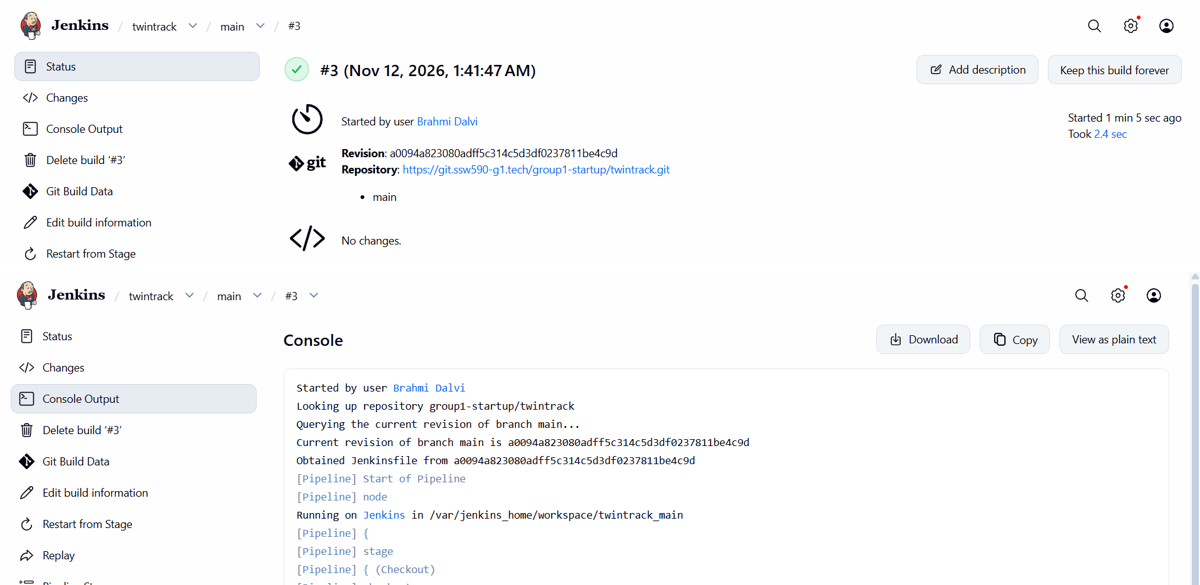
\includegraphics[width=0.9\linewidth]{evidence/169-jenkins-twintrack-main-build-3-success-2-4-s-and-console-running-on-controller-bd-2026-11-12.png}
\caption{Jenkins build \#3 of \texttt{twintrack/main} (Nov 12, 2026, 1:41:47 AM server time): SUCCESS, took 2.4~s, and its console, \texttt{Running on Jenkins in /var/jenkins\_home/workspace/twintrack\_main}, the controller.}
\label{Fig:E169}
\end{figure}

\paragraph{Observation.} The Jenkins probe duration shows one sample of about 4~s (above the 3~s red line) at about 16:25~EST on November 11. Its cause was not investigated; it is reported here instead of being hidden.

% ===== BD region: row 6 =====
% Region: sreAlerts (single owner; edit only your own region)
\section{Alerts (15 points)}\label{Section:sreAlerts}
\textbf{Owner:} BD. \textbf{Status:} both rules fired, delivered and resolved on November 11, 2026 \StatusPass.

\paragraph{Contact point and routing.} One contact point, \texttt{team-alerts}, uses Grafana's dedicated \emph{Discord} integration (no SMTP is needed)
and posts to a private Discord channel that both team members can read; resolved notifications stay on. The channel's webhook URL is a secret: it was
pasted only into Grafana, is stored in Grafana's volume, and is in no repository, screenshot or this PDF (\FigRef{149}; Grafana hides it). The default
notification policy sends everything to \texttt{team-alerts} (the built-in contact point \texttt{empty} has no integration and is unused), groups by folder and alert
name, waits 30~s before the first message, 1~minute before updates, and repeats every 4~hours (\FigRef{151}). A test message arrived in Discord (\FigRef{150}),
which proves delivery only; the rule tests below prove the queries, thresholds and routing.

\begin{figure}[htbp]
\centering
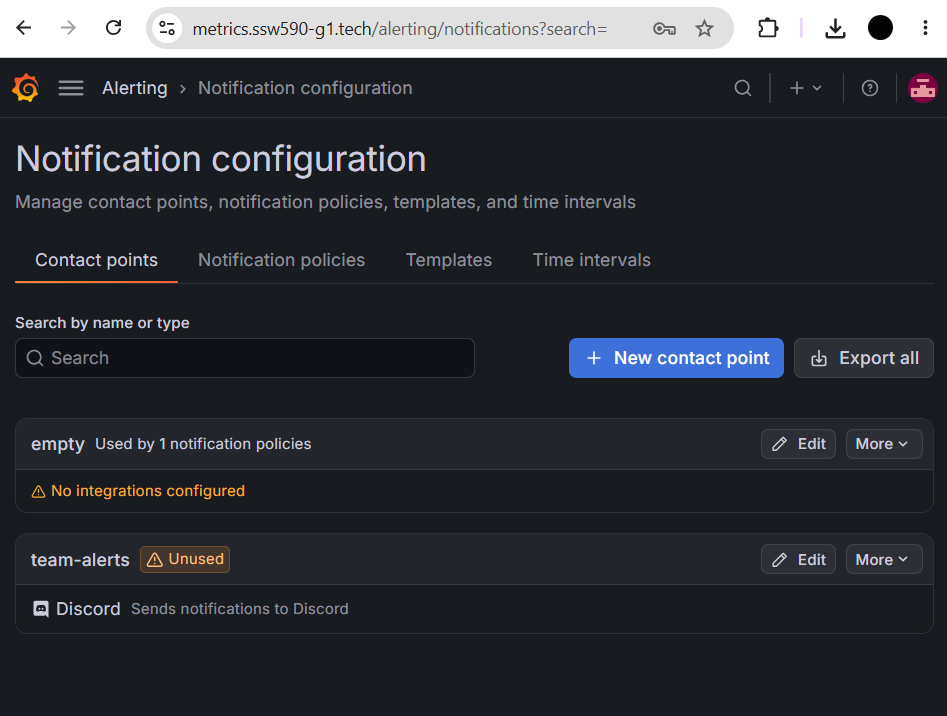
\includegraphics[width=0.8\linewidth]{evidence/149-grafana-contact-point-team-alerts-discord-saved-bd-2026-11-11.png}
\caption{Contact points: \texttt{team-alerts} with one Discord integration (the webhook URL is not shown); \texttt{empty} has no integrations.}
\label{Fig:E149}
\end{figure}

\begin{figure}[htbp]
\centering
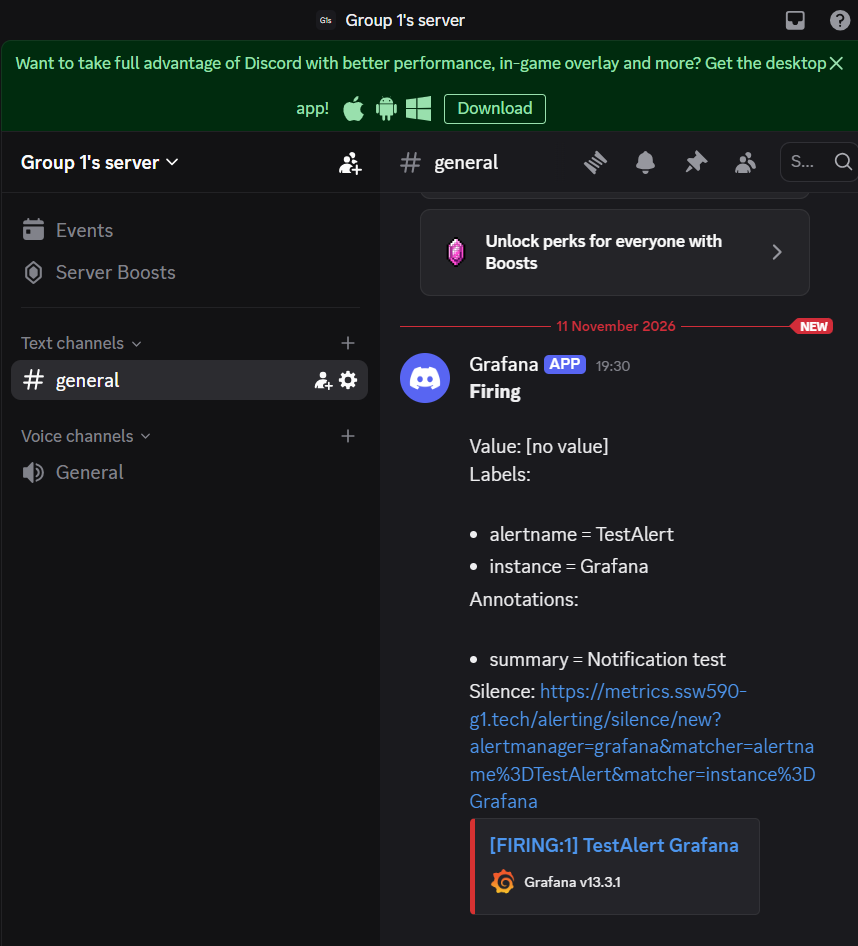
\includegraphics[width=0.8\linewidth]{evidence/150-discord-contact-point-test-notification-received-bd-2026-11-11.png}
\caption{Grafana's test notification in the Discord channel, November 11, 2026, 19:30 EST.}
\label{Fig:E150}
\end{figure}

\begin{figure}[htbp]
\centering
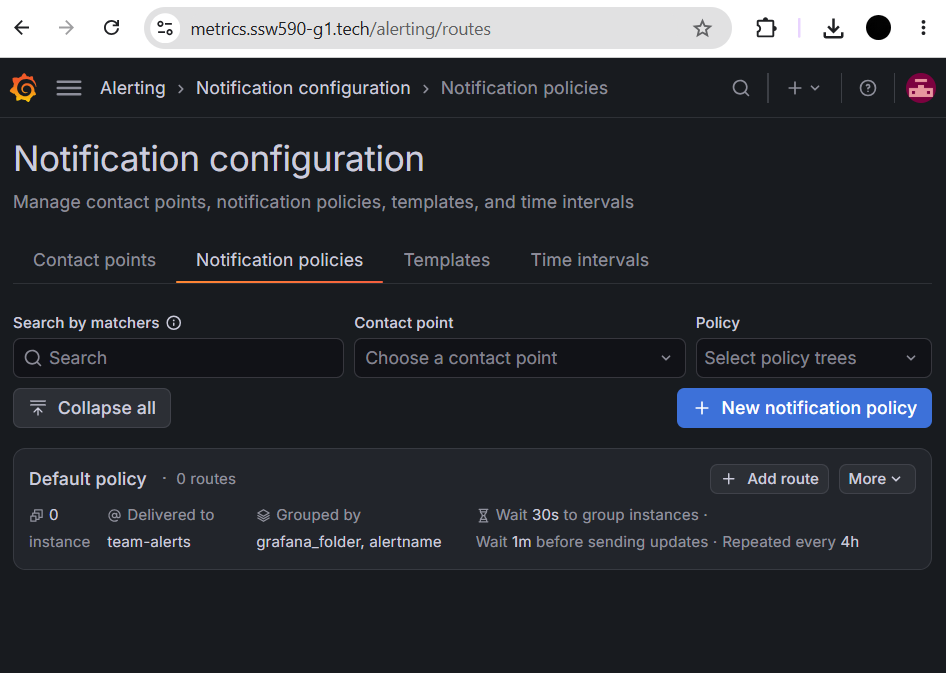
\includegraphics[width=0.8\linewidth]{evidence/151-grafana-default-notification-policy-team-alerts-timing-bd-2026-11-11.png}
\caption{Default notification policy: delivered to \texttt{team-alerts}, grouped by \texttt{grafana\_folder} and \texttt{alertname}, group wait 30~s, group interval 1~m, repeat 4~h.}
\label{Fig:E151}
\end{figure}

\paragraph{The two rules.} Both rules are Grafana-managed, live in the folder \emph{Group 1}, and are exported as YAML
(\texttt{config/monitoring/grafana/alert-rules.yaml}) so that they can be restored.

\begin{tabularx}{\linewidth}{L{2.6cm}YY}
\caption{Alert rules: owner, severity, query, threshold, timing, no-data policy\label{Table:SreRules}}\\
\toprule \textbf{Item} & \textbf{\texttt{https-service-down}} & \textbf{\texttt{root-disk-below-15-percent}}\\ \midrule
\endfirsthead
\toprule \textbf{Item} & \textbf{\texttt{https-service-down}} & \textbf{\texttt{root-disk-below-15-percent}}\\ \midrule
\endhead \bottomrule \endlastfoot
Owner, severity & Brahmi Dalvi; \texttt{critical} & Brahmi Dalvi; \texttt{warning}\\
Query & \texttt{\small probe\_success\{job="https"\}}: one alert per \texttt{instance} (Gitea, Jenkins) & the root-filesystem free-percentage query of panel~3 (\texttt{/dev/nvme0n1p1}, xfs only)\\
Threshold & below 1 & below 15 (percent free)\\
Evaluation, pending & every 30~s; pending 1~minute & every 1~minute; pending 5~minutes\\
No data, error & \texttt{NoData} and \texttt{Error}: each raises its own alert to \texttt{team-alerts}, so a missing series or failed collection is reported and never read as healthy & the same\\
Summary & \texttt{\{\{ \$labels.instance \}\} failed its HTTPS probe for at least 1 minute} & Root filesystem has less than 15\% free\\
Operator response & check the container (\texttt{docker ps}, \texttt{docker logs}), HTTPS from outside, Caddy and the certificate; restart the container; see Section~\ref{Section:sreIncident} & \texttt{docker system df}; remove unused images only after checking they are not the runner's image; check Prometheus (1~GB cap) and logs; never delete volumes\\
Runbook link & \Todo{runbook link to the incident section} & the same\\
\end{tabularx}

\FigRef{152} to \FigRef{155} show both saved rules (state, query, threshold, pending period, no-data and error states, annotations).

\begin{figure}[htbp]
\centering
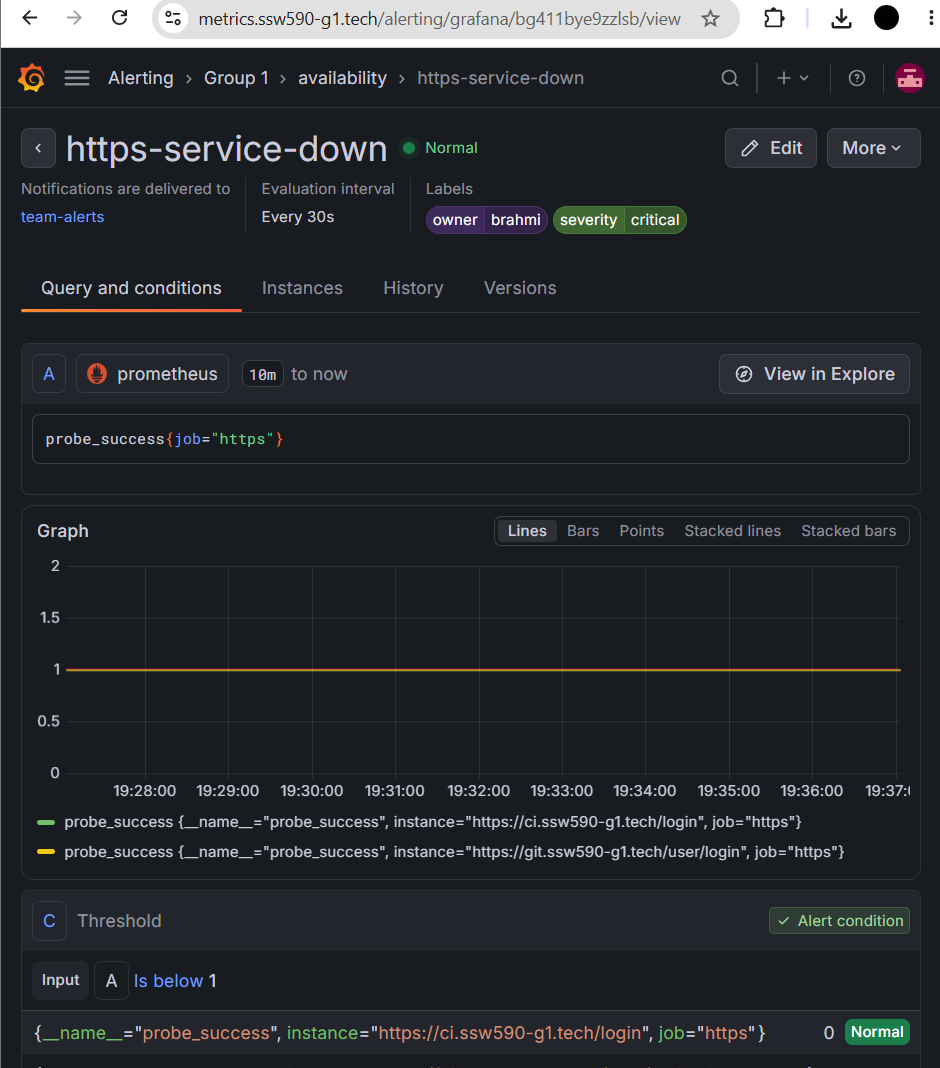
\includegraphics[width=0.85\linewidth]{evidence/152-grafana-alert-rule-https-service-down-query-threshold-labels-bd-2026-11-11.png}
\caption{Rule \texttt{https-service-down}: query, threshold ``below 1'', labels \texttt{owner} and \texttt{severity}, notifications to \texttt{team-alerts}.}
\label{Fig:E152}
\end{figure}

\begin{figure}[htbp]
\centering
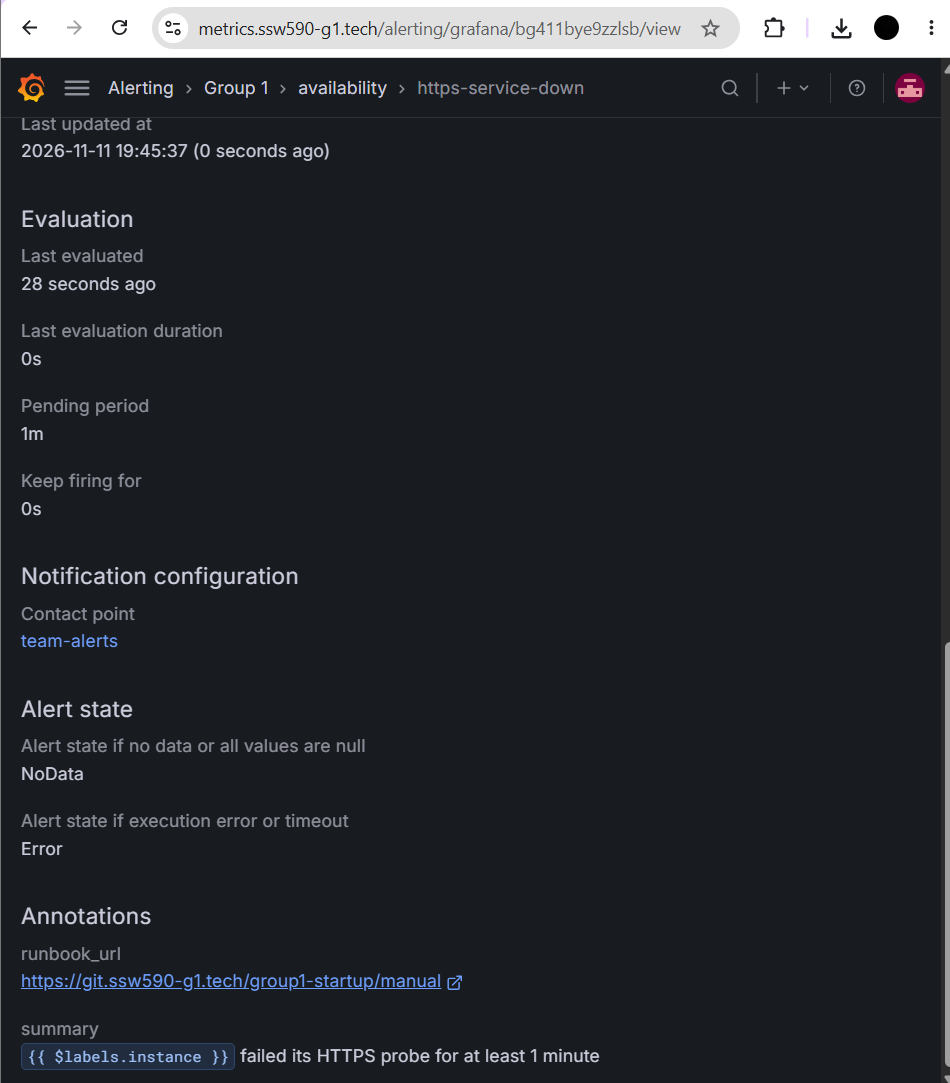
\includegraphics[width=0.85\linewidth]{evidence/153-grafana-alert-rule-https-service-down-pending-nodata-error-summary-runbook-bd-2026-11-11.png}
\caption{The same rule, lower part: pending 1~m, no data \texttt{NoData}, error \texttt{Error}, \texttt{runbook\_url} and \texttt{summary}.}
\label{Fig:E153}
\end{figure}

\begin{figure}[htbp]
\centering
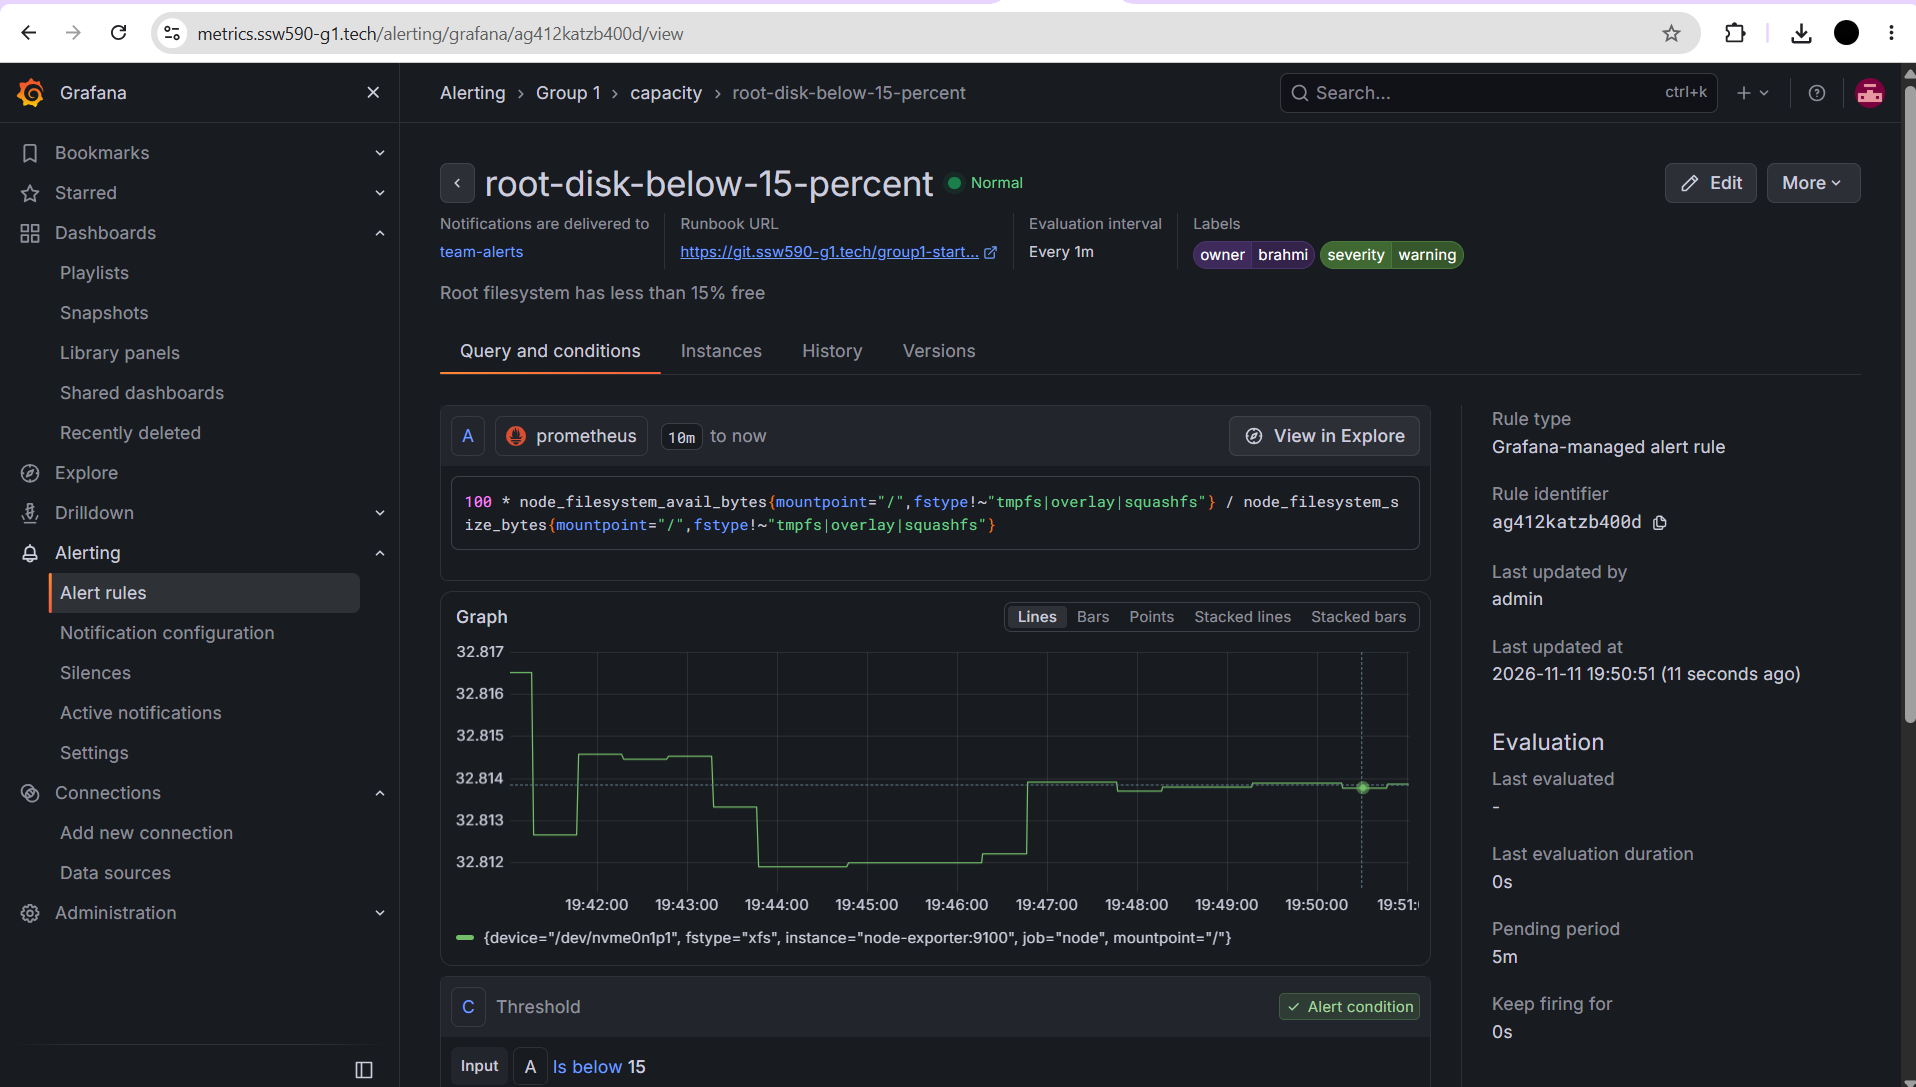
\includegraphics[width=0.85\linewidth]{evidence/154-grafana-alert-rule-root-disk-below-15-percent-query-labels-graph-bd-2026-11-11.png}
\caption{Rule \texttt{root-disk-below-15-percent}: query for the xfs root, graph at about 32.8\%, threshold ``below 15''.}
\label{Fig:E154}
\end{figure}

\begin{figure}[htbp]
\centering
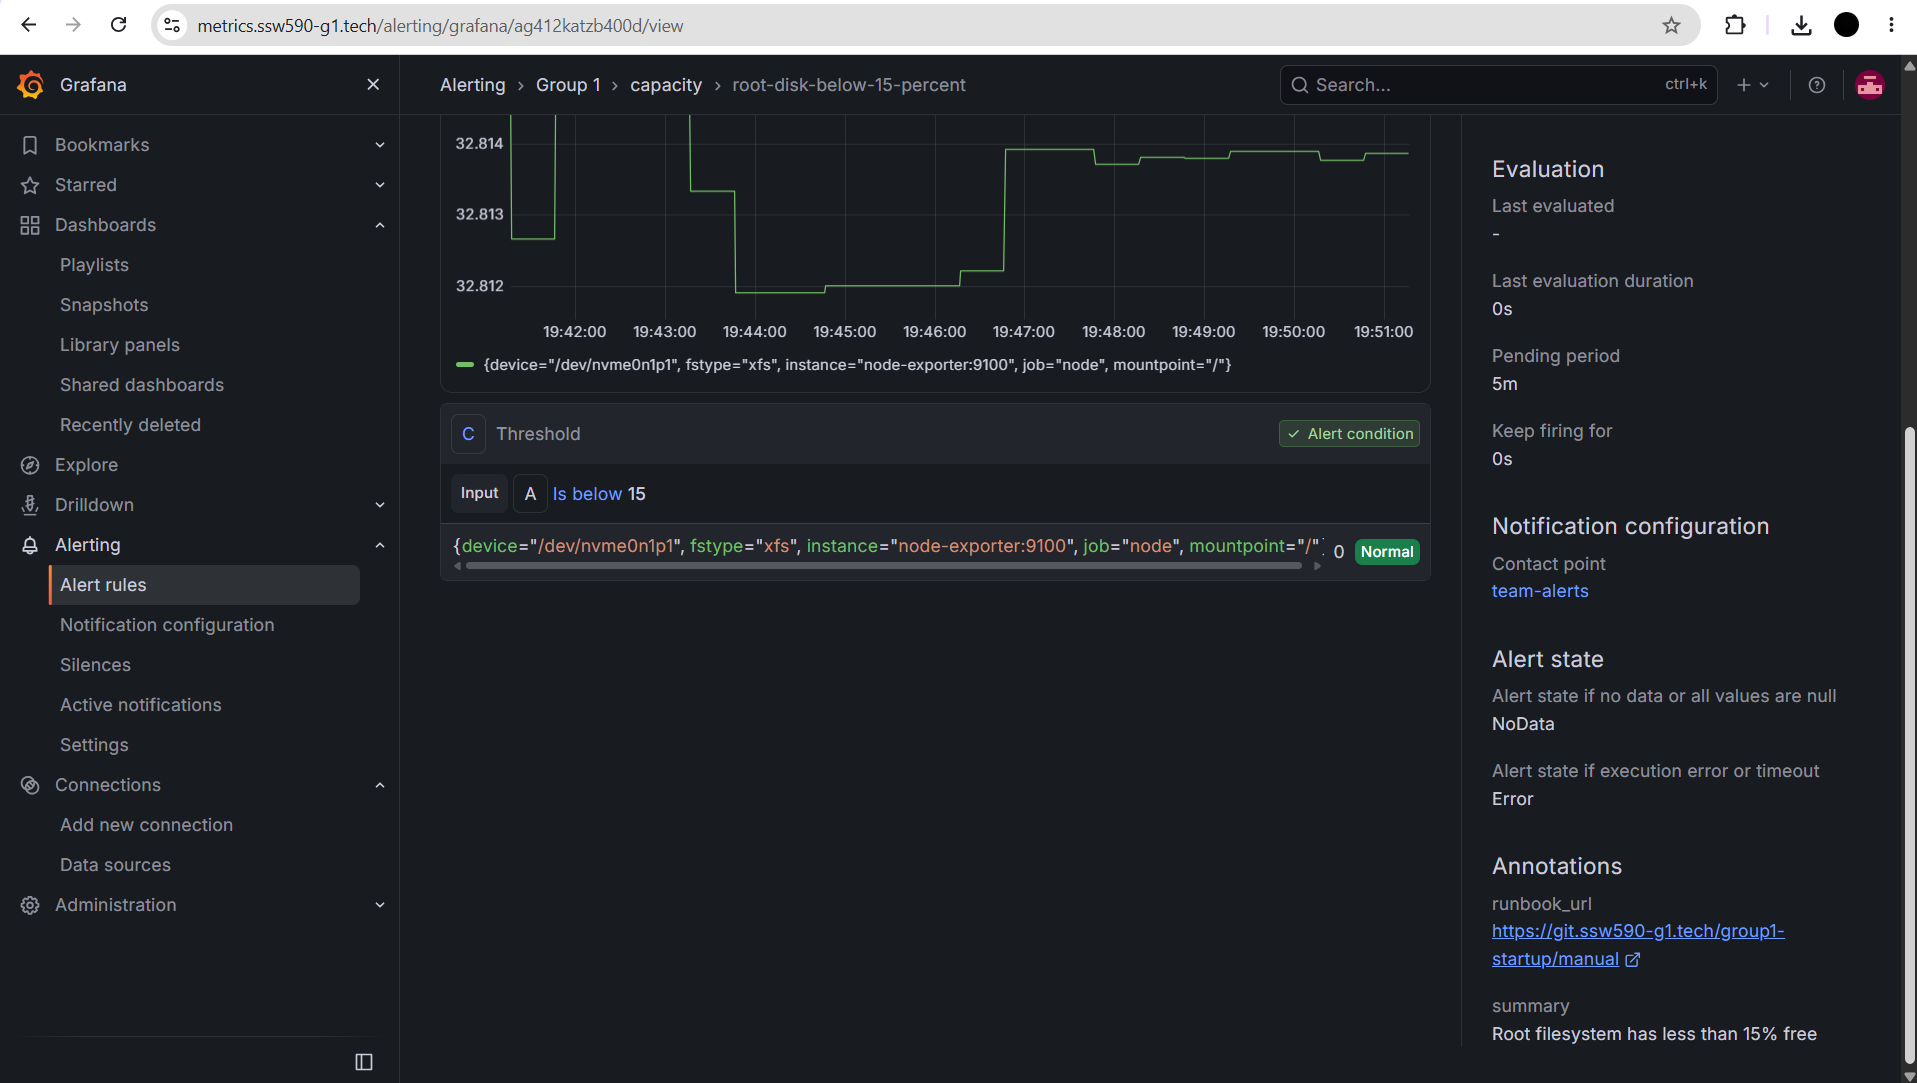
\includegraphics[width=0.85\linewidth]{evidence/155-grafana-alert-rule-root-disk-below-15-percent-pending-nodata-error-annotations-bd-2026-11-11.png}
\caption{The same rule, lower part: pending 5~m, \texttt{NoData}, \texttt{Error}, \texttt{runbook\_url}, \texttt{summary}.}
\label{Fig:E155}
\end{figure}

\paragraph{Test 1: host capacity, with a temporary threshold.} The disk was never filled. On November 11, 2026 the threshold was raised from 15 to 55 percent
(the disk had about 33\% free) at 20:02:10~EST; the rule went to Pending at 20:02:30 and to Alerting after exactly the 5-minute pending period at 20:07:30; the Discord message arrived at 20:08
(\FigRef{157}); the threshold was restored to 15 at 20:15:20, the rule was Normal at once, and the Resolved message arrived at 20:16 (\ListRef{162}). The Resolved message says
\texttt{grafana\_state\_reason = Updated}: the alert cleared because the rule was edited back, which is the planned way to test resolution. The final threshold is 15.

\begin{longlisting}
\inputminted[fontsize=\scriptsize]{text}{evidence/162-disk-alert-test-timeline-threshold-55-then-restored-15-bd-2026-11-11.txt}
\caption{Real timeline of the disk-capacity test: raised to 55, Pending, Firing, Discord, restored to 15, Normal, Resolved.}
\label{Listing:E162}
\end{longlisting}

\begin{figure}[htbp]
\centering
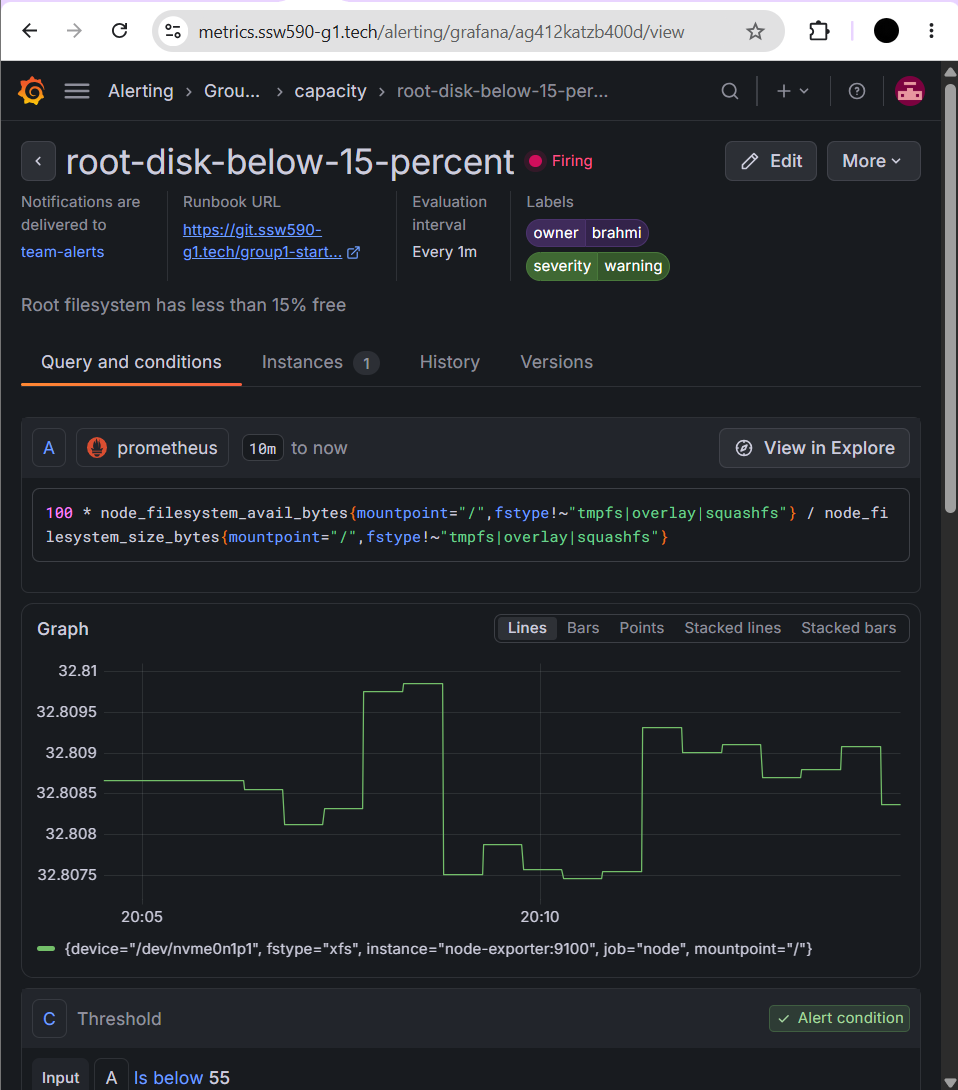
\includegraphics[width=0.8\linewidth]{evidence/157-grafana-disk-rule-firing-threshold-55-bd-2026-11-11.png}
\caption{Disk rule Firing with the temporary threshold 55, 20:08 EST.}
\label{Fig:E157}
\end{figure}

\begin{figure}[htbp]
\centering
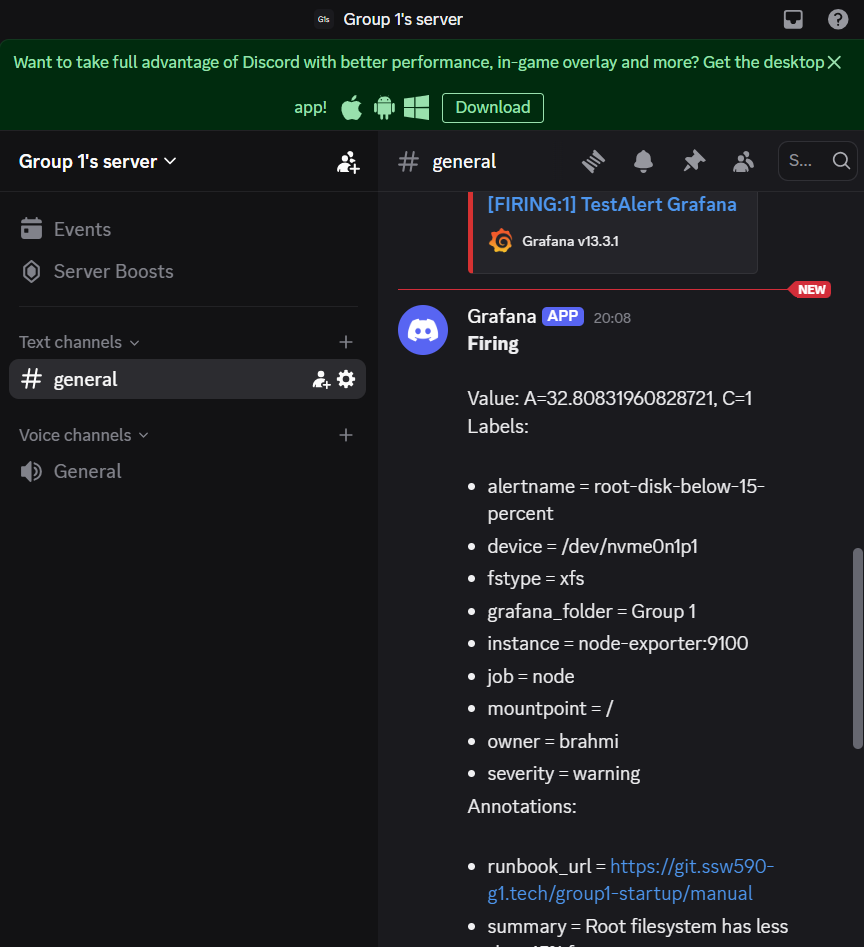
\includegraphics[width=0.8\linewidth]{evidence/158-discord-disk-alert-firing-notification-20-08-bd-2026-11-11.png}
\caption{The Discord Firing message for the disk rule, 20:08 EST.}
\label{Fig:E158}
\end{figure}

\begin{figure}[htbp]
\centering
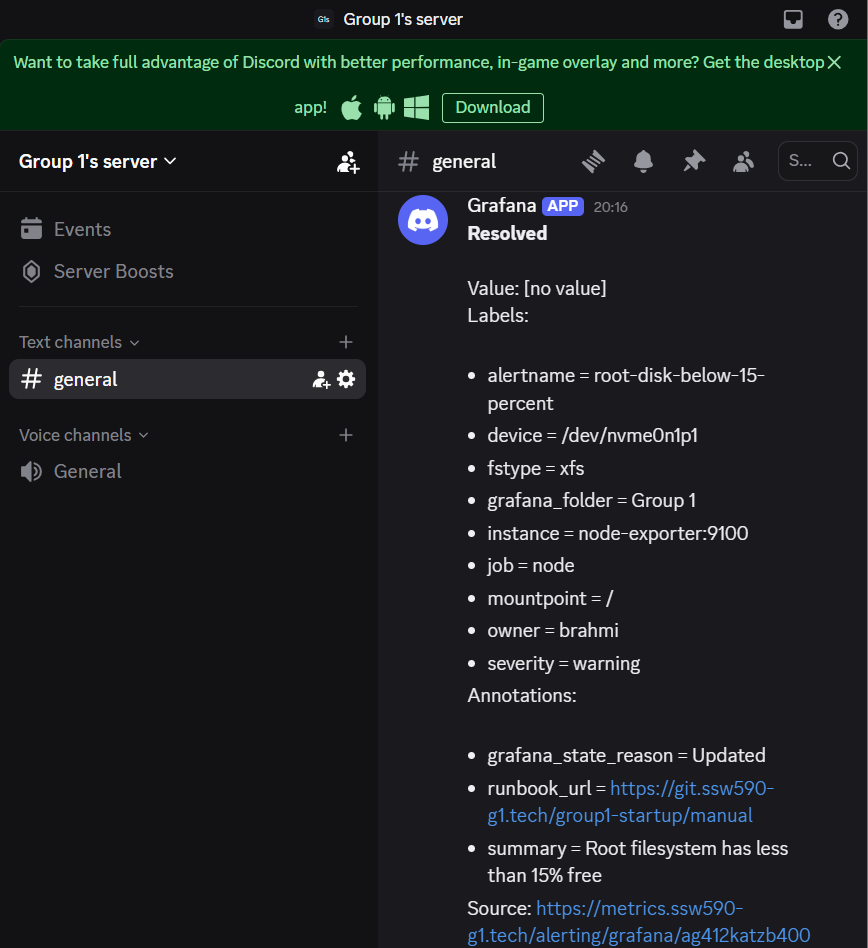
\includegraphics[width=0.8\linewidth]{evidence/160-discord-disk-alert-resolved-notification-20-16-bd-2026-11-11.png}
\caption{The Discord Resolved message, 20:16 EST, after the threshold was restored to 15.}
\label{Fig:E160}
\end{figure}

\paragraph{Test 2: service availability.} The second rule was tested by the controlled Jenkins outage (Section~\ref{Section:sreIncident}): it went Pending at 20:25:10~EST, Firing at 20:26:10, a Discord message
arrived at 20:26 (\FigRef{164}), and after the restart the rule was Normal at 20:28:10 with a Resolved message at 20:28 (\FigRef{165}, \FigRef{163}).

% ===== BD region: row 7 =====
% Region: sreIncident (single owner; edit only your own region)
\section{Controlled incident and review (10 points)}\label{Section:sreIncident}
\textbf{Owner:} BD, with SD recording. \textbf{Status:} outage run and verified November 11, 2026; blameless review and issues \StatusPending.

\paragraph{Exercise.} BD and SD agreed, both being on campus, to stop only the Jenkins container for about three minutes. No build was running. Gitea and monitoring stayed up; no volume was
touched and the instance was not stopped. BD ran \texttt{docker stop jenkins} and, after the Discord message, \texttt{docker start jenkins} in an SSH session, each with the time printed by \texttt{date -u}.

\begin{tabularx}{\linewidth}{L{2.4cm}L{1.9cm}Y}
\caption{Incident timeline, November 11 to 12, 2026\label{Table:SreTimeline}}\\
\toprule \textbf{UTC} & \textbf{EST} & \textbf{Event}\\ \midrule
\endfirsthead
\toprule \textbf{UTC} & \textbf{EST} & \textbf{Event}\\ \midrule
\endhead \bottomrule \endlastfoot
01:24:25 & 20:24:25 & Injection: \texttt{docker stop jenkins}\\
01:24:49 & 20:24:49 & First failing probe (24~s later)\\
01:25:10 & 20:25:10 & Rule Pending\\
01:26:10 & 20:26:10 & Rule Firing (after the 1-minute pending period)\\
about 01:26 & 20:26 & Discord Firing message received; read, then acknowledged by restarting (exact time not recorded)\\
01:27:25 & 20:27:25 & Restart: \texttt{docker start jenkins} (3~min 0~s after the stop)\\
01:27:49 & 20:27:49 & First successful probe\\
01:28:10 & 20:28:10 & Rule Normal\\
about 01:28 & 20:28 & Discord Resolved message\\
01:29:12 & 20:29:12 & Jenkins \texttt{main} build \#2 started by BD: SUCCESS in 7.9~s\\
01:29:14--01:29:20 & & Gitea receives the \texttt{twintrack/pipeline/head} status for \texttt{a0094a8}: pending, pending, success\\
\end{tabularx}

\paragraph{Detection and restoration.} From the stop to the first failing probe: 24~s (at most one 30~s scrape). From the stop to the rule's Firing state: 1~min 45~s. From the stop to the Discord message: about 2~min 15~s
(Discord shows only the minute; the 30~s group wait follows Firing). From the stop to the first successful probe: 3~min 24~s; from the restart to it: 24~s (Jenkins' own start-up is about 13~s). From the first
successful probe to Normal: 21~s. The settings (scrape 30~s, evaluation 30~s, pending 60~s, group wait 30~s) allow at most 2~min 30~s before a message, so the observed delay is as configured.
Gitea stayed at 1 in all 18 samples around the outage while 6 Jenkins samples failed (\ListRef{167}).

\begin{longlisting}
\inputminted[fontsize=\scriptsize]{text}{evidence/167-controlled-jenkins-outage-timeline-and-recovery-checks-bd-2026-11-11.txt}
\caption{Real timeline of the controlled Jenkins outage with the raw probe samples, the calculated times and the recovery checks.}
\label{Listing:E167}
\end{longlisting}

\begin{figure}[htbp]
\centering
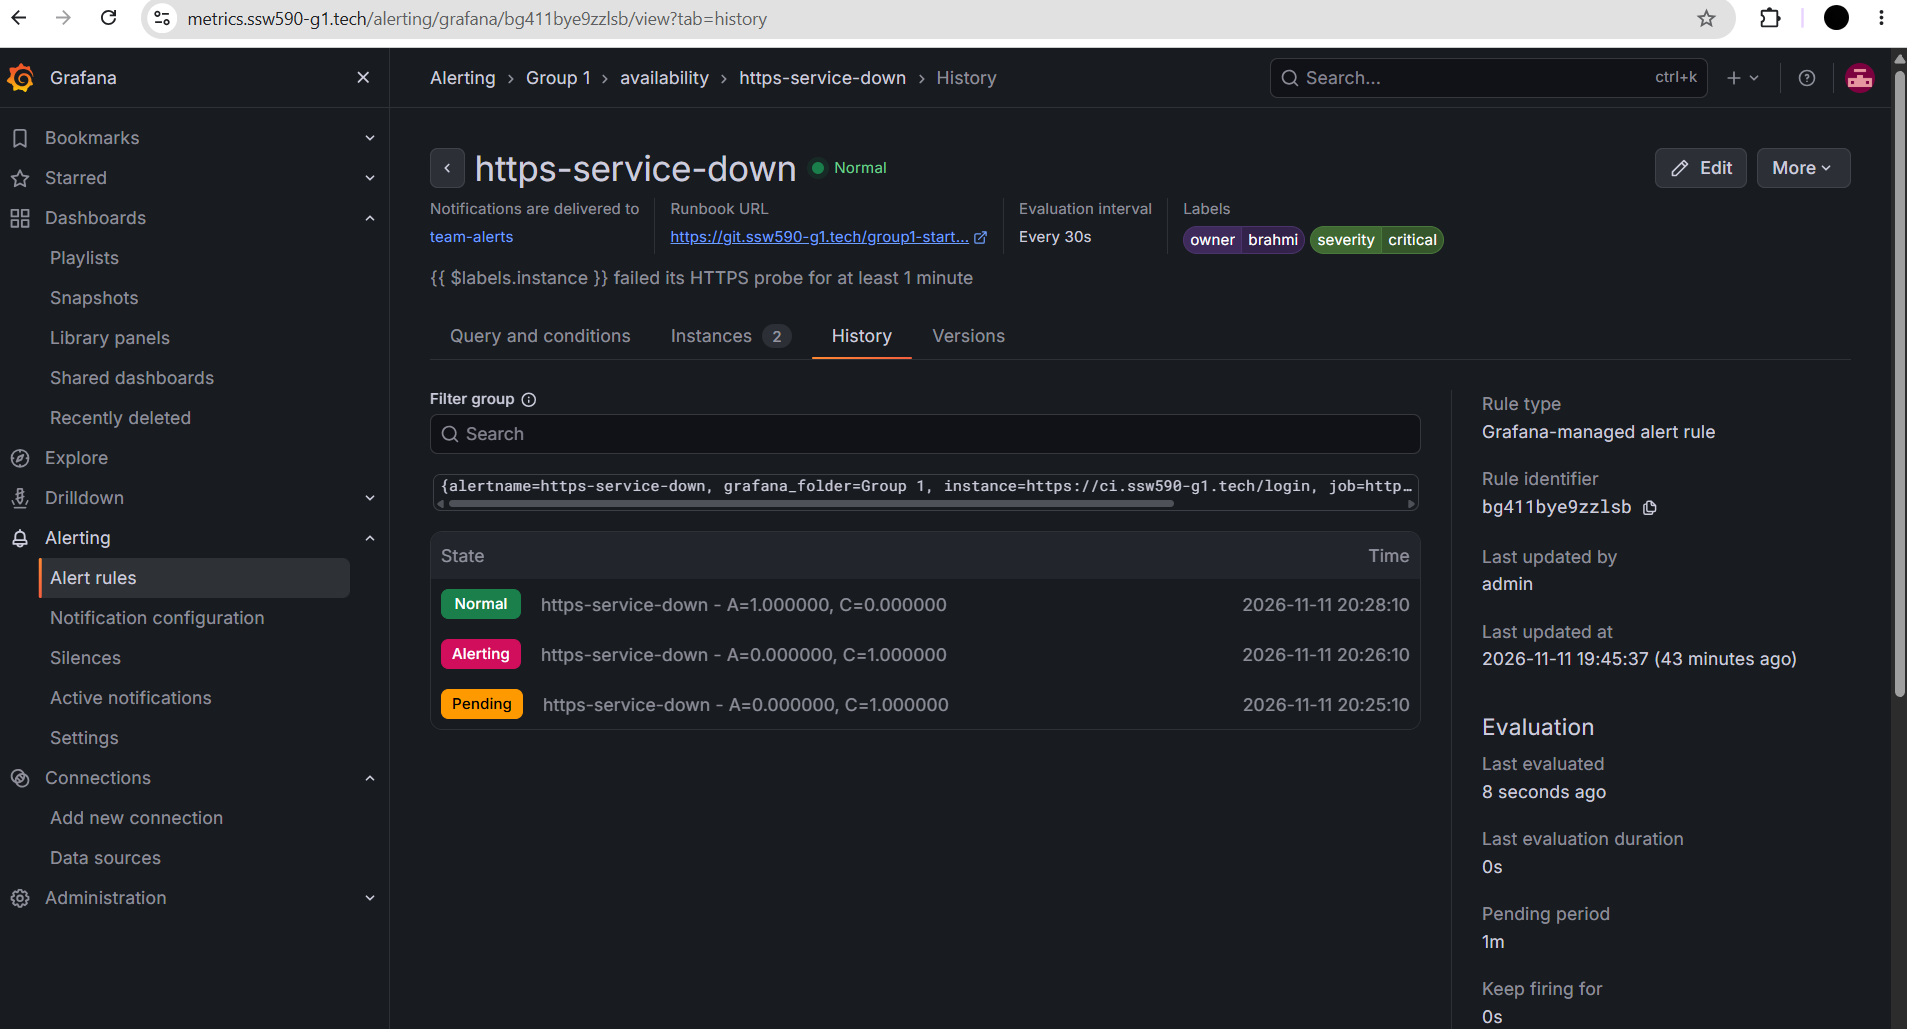
\includegraphics[width=\linewidth]{evidence/163-grafana-jenkins-outage-rule-history-pending-alerting-normal-bd-2026-11-11.png}
\caption{History of the rule for the Jenkins instance: Pending 20:25:10, Alerting 20:26:10, Normal 20:28:10 (EST).}
\label{Fig:E163}
\end{figure}

\begin{figure}[htbp]
\centering
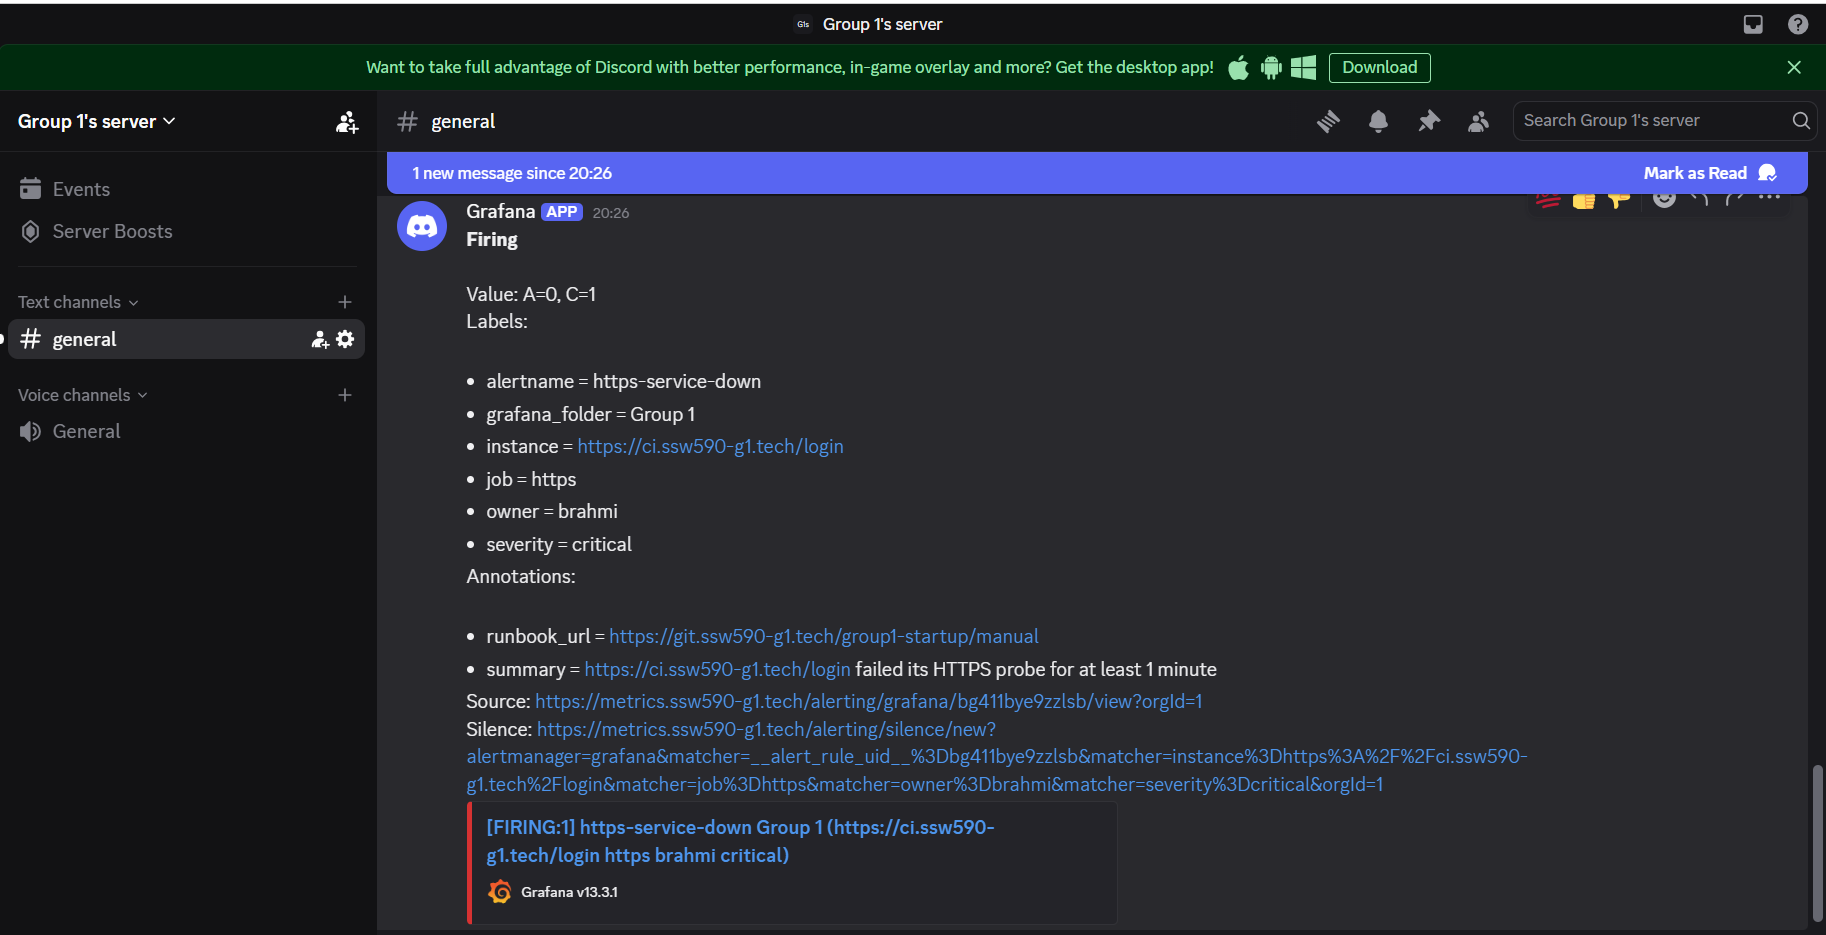
\includegraphics[width=\linewidth]{evidence/164-discord-jenkins-outage-firing-notification-20-26-bd-2026-11-11.png}
\caption{Discord Firing message for \texttt{https://ci.ssw590-g1.tech/login}, 20:26 EST.}
\label{Fig:E164}
\end{figure}

\begin{figure}[htbp]
\centering
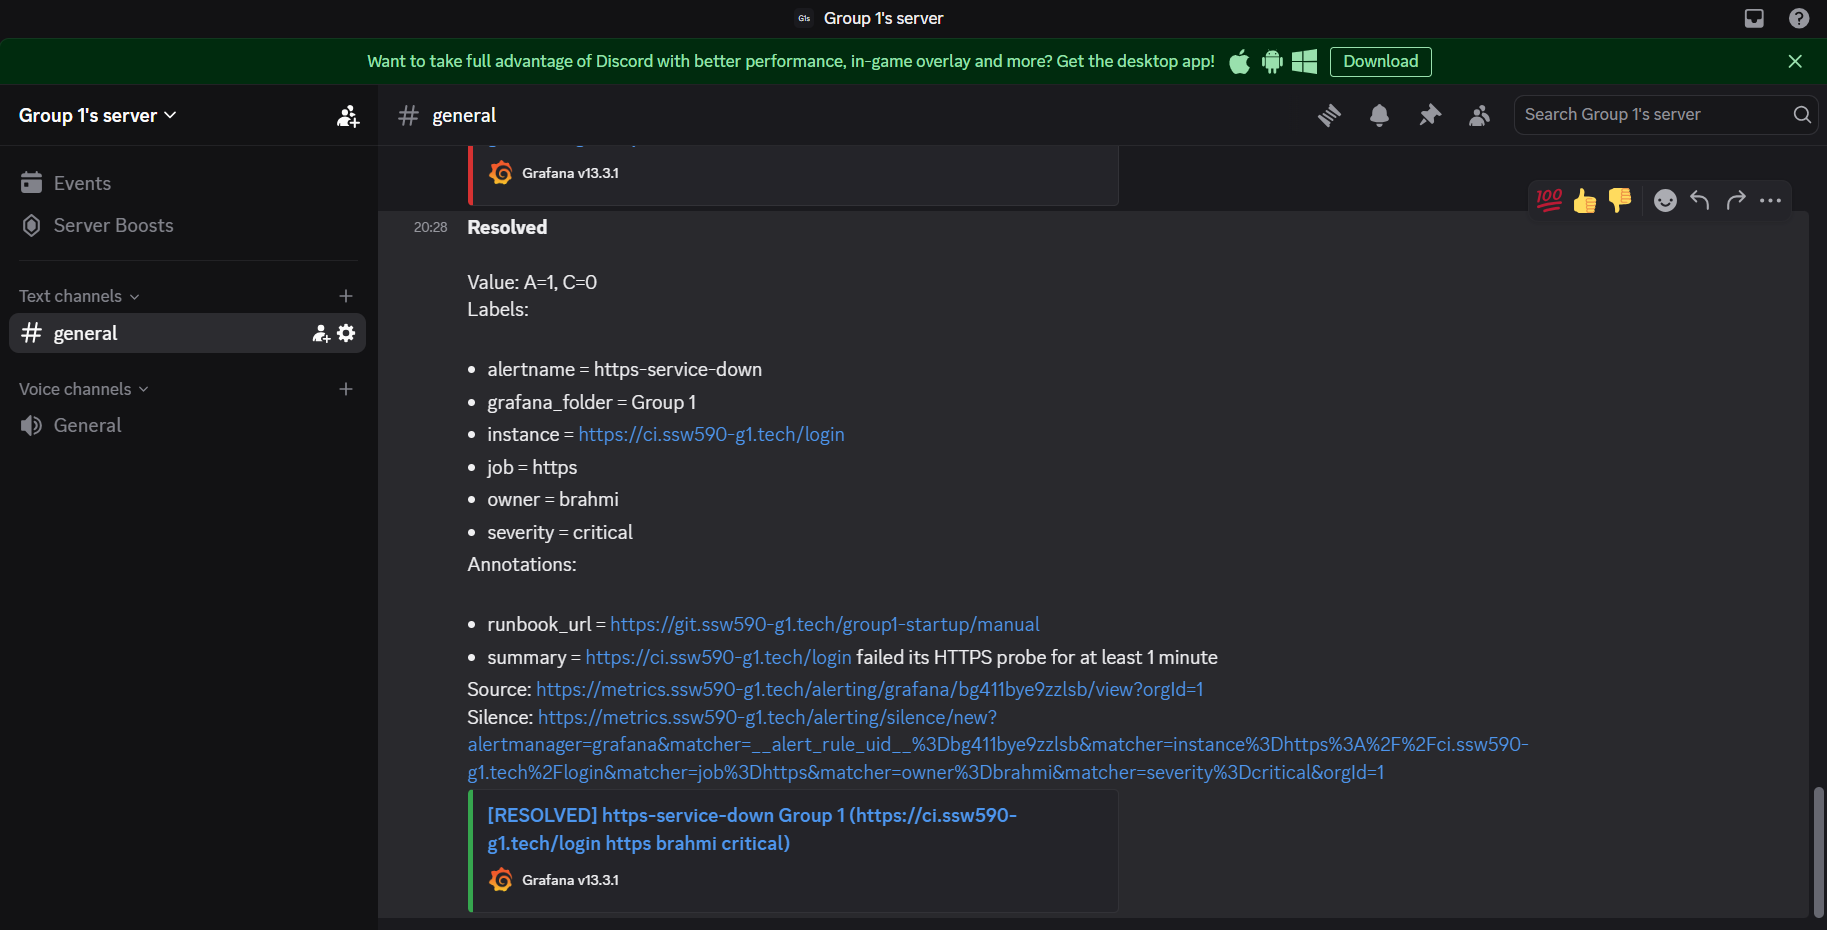
\includegraphics[width=\linewidth]{evidence/165-discord-jenkins-outage-resolved-notification-20-28-bd-2026-11-11.png}
\caption{Discord Resolved message, 20:28 EST.}
\label{Fig:E165}
\end{figure}

\paragraph{Verification.} After the restart, Jenkins' login page answered, a pipeline run of \texttt{main} passed (\FigRef{166}), and the commit status of that run reached Gitea, so the Jenkins-to-Gitea status path works again.
The Prometheus and Grafana restart test followed and is described with the deployment (Section~\ref{Section:sreDeployment}); \Todo{link to SD's restart-test listing}.

\begin{figure}[htbp]
\centering
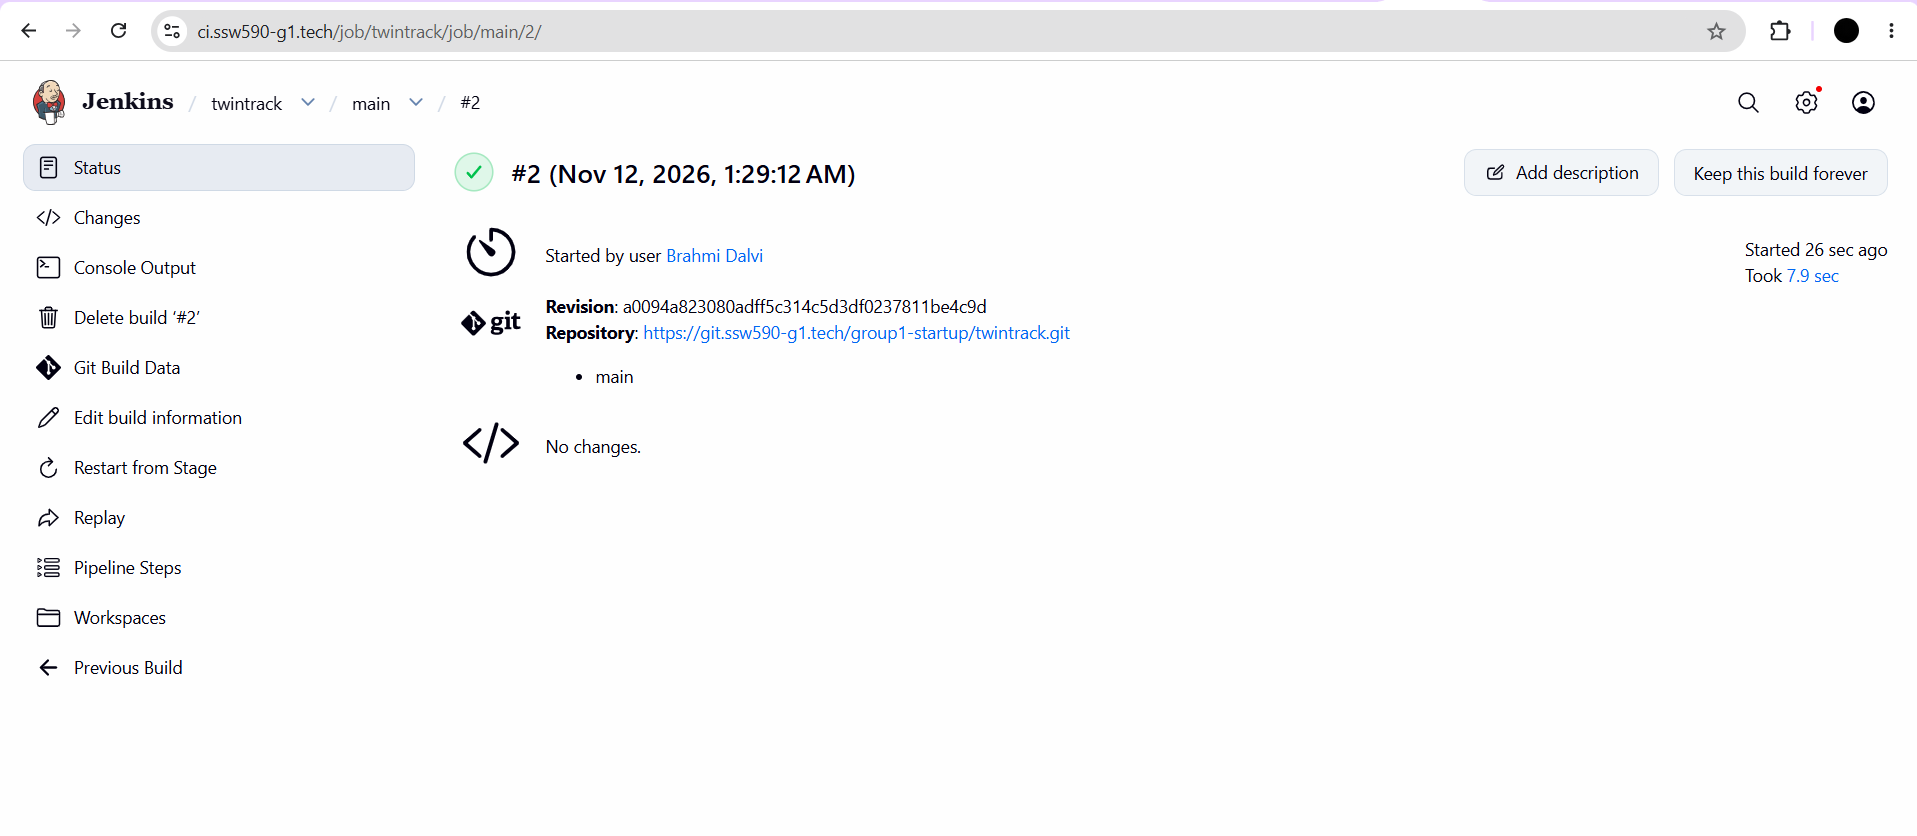
\includegraphics[width=\linewidth]{evidence/166-jenkins-twintrack-main-build-2-success-after-outage-bd-2026-11-11.png}
\caption{Jenkins \texttt{twintrack/main} build \#2 after the outage, Nov 12, 2026, 1:29:12 AM server time (UTC): SUCCESS in 7.9~s.}
\label{Fig:E166}
\end{figure}

\paragraph{Compared with Chapter~4.} In Chapter~\ref{Chapter:Jenkins} a \emph{bad commit} failed its tests and Gitea's merge gate refused the merge, while Jenkins itself was healthy.
Here the commit was fine and the \emph{CI service} was down: nothing failed in Jenkins' tests, no commit status changed, and only monitoring noticed. The two checks cover different failures and neither replaces the other.

\paragraph{Blameless review.} \Todo{impact (Jenkins unavailable for 3 min 24 s as seen by probes; team users only), cause (deliberate injection), response, measurement gaps}.
Measurement gaps already known: one probe location only, and it runs on the same host, so an outage of the whole host would also stop monitoring; probes every 30~s cannot see shorter outages; the acknowledgement time was not recorded.

\paragraph{Improvement issues.} \Todo{two prioritized issues in Gitea with owners: (1) the shared-server limitation, an off-host probe; (2) a backup of the Grafana and Prometheus volumes or a scheduled notification test; link both}.

% ===== BD region: row 8 =====
% Region: sreManual (single owner; edit only your own region)
\section{Manual changes in this version (10 points)}\label{Section:sreManual}
\textbf{Owner:} BD. \textbf{Status:} \StatusPending.

\Todo{version 1.3 and date in devopsITManual.tex; dated entry in devopsDocumentHistory.tex; list here the Hosts and Passwords changes (metrics host and DNS record, four monitoring containers and their private ports, Grafana administrator hint, Discord webhook hint, SSH and team-address entries for the campus address); glossary terms SRE, SLI, SLO, SLA, error budget, Prometheus, Grafana, exporter, probe; citations; AI and reuse attribution; link to the successful PDF build and the reviewed final commit; final scan for TODO and undefined references.}
